%
% hatpsi.tex -- Zulässigkeitsbedingung für Haar Wavelet
%
% (c) 2019 Prof Dr Andreas Müller, Hochschule Rapperswil
%
\documentclass[tikz]{standalone}
\usepackage{amsmath}
\usepackage{times}
\usepackage{txfonts}
\usepackage{pgfplots}
\usepackage{csvsimple}
\usetikzlibrary{arrows,intersections,math}
\begin{document}
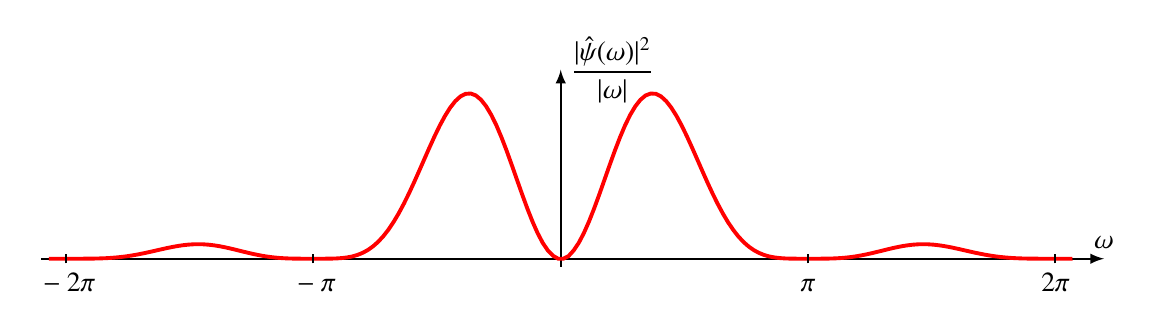
\begin{tikzpicture}[>=latex]

\draw[->,line width=0.7pt] (-6.6,0)--(6.9,0) coordinate[label={$\omega$}];
\draw[->,line width=0.7pt] (0,-0.1)--(0,2.4) coordinate[label={right:$\displaystyle\frac{|\hat{\psi}(\omega)|^2}{|\omega|}$}];

\def\a{1}
\def\A{4}
\def\s{0.06}

\draw[line width=1.4pt,color=red]
	plot[domain=-6.5:6.5,samples=200]
		({\x},{\A*sin(\a*180*\x/3.1415)^4/(\a*\x)^2});

\draw[line width=0.7pt] ({1*3.1415},-\s)--({1*3.1415},\s);
\draw[line width=0.7pt] ({2*3.1415},-\s)--({2*3.1415},\s);
\draw[line width=0.7pt] ({-1*3.1415},-\s)--({-1*3.1415},\s);
\draw[line width=0.7pt] ({-2*3.1415},-\s)--({-2*3.1415},\s);

\node at ({1*3.1415},-\s) [below] {$\mathstrut\pi$};
\node at ({2*3.1415},-\s) [below] {$\mathstrut2\pi$};
\node at ({-1*3.1415},-\s) [below] {$\mathstrut-\pi$};
\node at ({-2*3.1415},-\s) [below] {$\mathstrut-2\pi$};

\end{tikzpicture}
\end{document}

